El control de versiones consiste en tener todas las versiones de código que se han generado etiquetadas, de forma que se pueda acceder a cualquier versión generada en cualquier momento. Esta es una base imprescindible para un proyecto de calidad, ya que permite trazar errores con mucha facilidad y es una salvaguarda ante fallos. Además, el control de versiones permite tener varias ramas de trabajo, separando el código de la rama de producción, la rama de desarrollo y las distintas ramas de los equipos y características que se están trabjando.

Hay muchas herramientas que permiten realizar este control de versiones y está sujeto a opinión cuál es mejor. Lo que no está sujeto a opinión es cuál se está utilizando más, lo cual se puede ver en gráficas como la figura \cref{fig:bd:source-control}, que nos facilita \citet{BDSRCMP}. Aparentemente el 70\% de los repositorios públicos está controlado mediante git. 

Otra ventaja de git es que es considerada la herramienta de alto rendimiento. Esto se puede ver también en la figura \cref{fig:g2:source-control}. El origen de esta figura, \citet{G2SRCMP}, nos permite además ir probando distintos parámetros, como el tamaño de la empresa. Y nos muestra que, en cualquier caso, git es la herramienta a elegir para el alto rendimiento.

Así que, con respecto al control de versiones, no hay duda de que git es la herramienta a elegir. Nos permite abarcar la mayoría de desarrollos públicos y es perfecto para el desarrollo de alto rendimiento que necesita un proyecto de calidad. Sin embargo, las decisiones no han acabado aquí. El control de versiones suele subirse a un servidor de repositorios -especialmente si pretende ser código libre-. Este proyecto va a ser código libre, de modo que se puedan proponer cambios y ramificar según distintas necesidades. Para esto, \citet{GHVSGL} explica de forma muy completa que, para proyectos de código abierto, Github es el que tiene mayor comunidad, así que va a tener com más facilidad una repercursión real.

Por tanto, han sido seleccionados git y Github para el control de versiones.

\begin{figure}
	\centering
	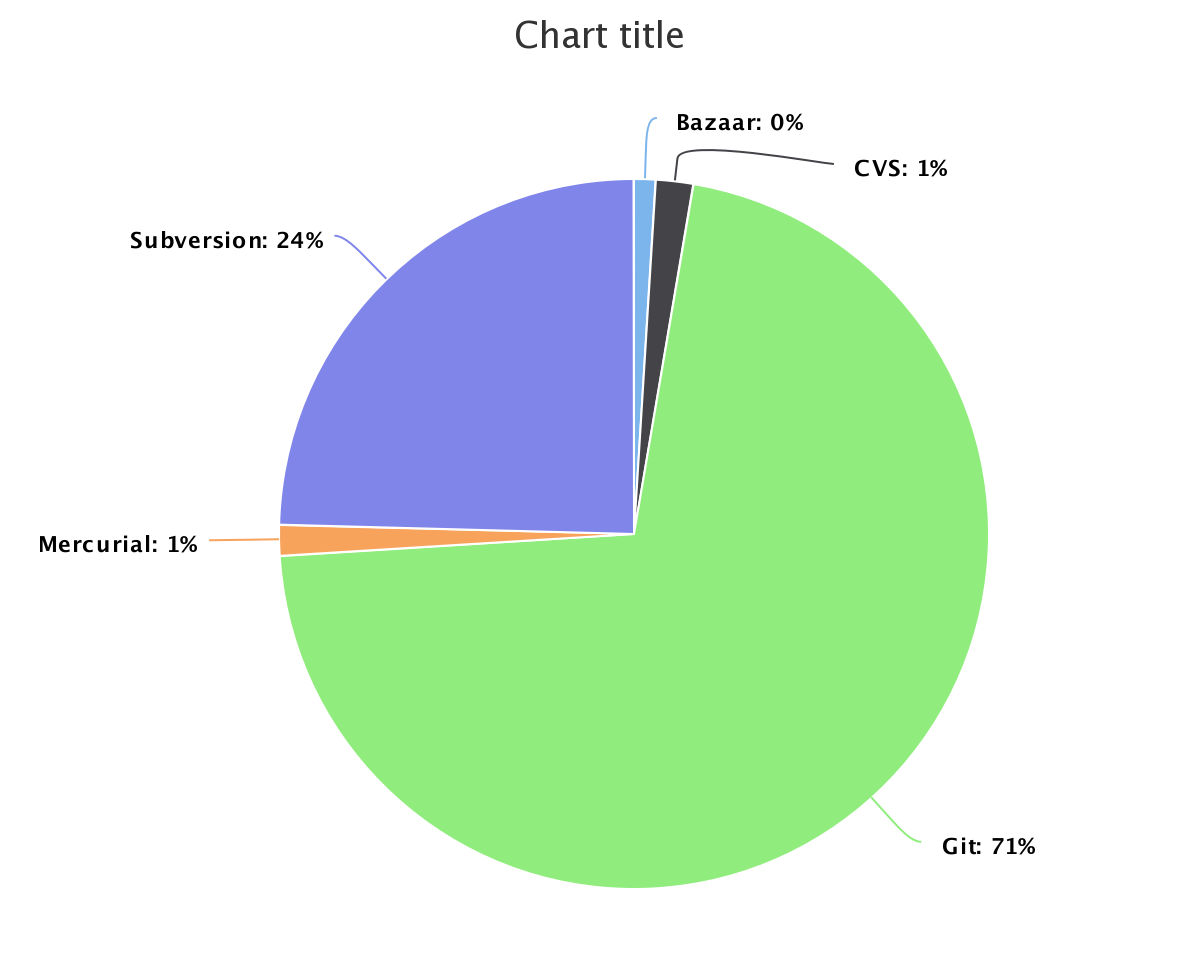
\includegraphics[width=\textwidth]{source-control.png}
	\caption{2019 - Compare Repositories}
	\label{fig:bd:source-control}
\end{figure}

\begin{figure}
	\centering
	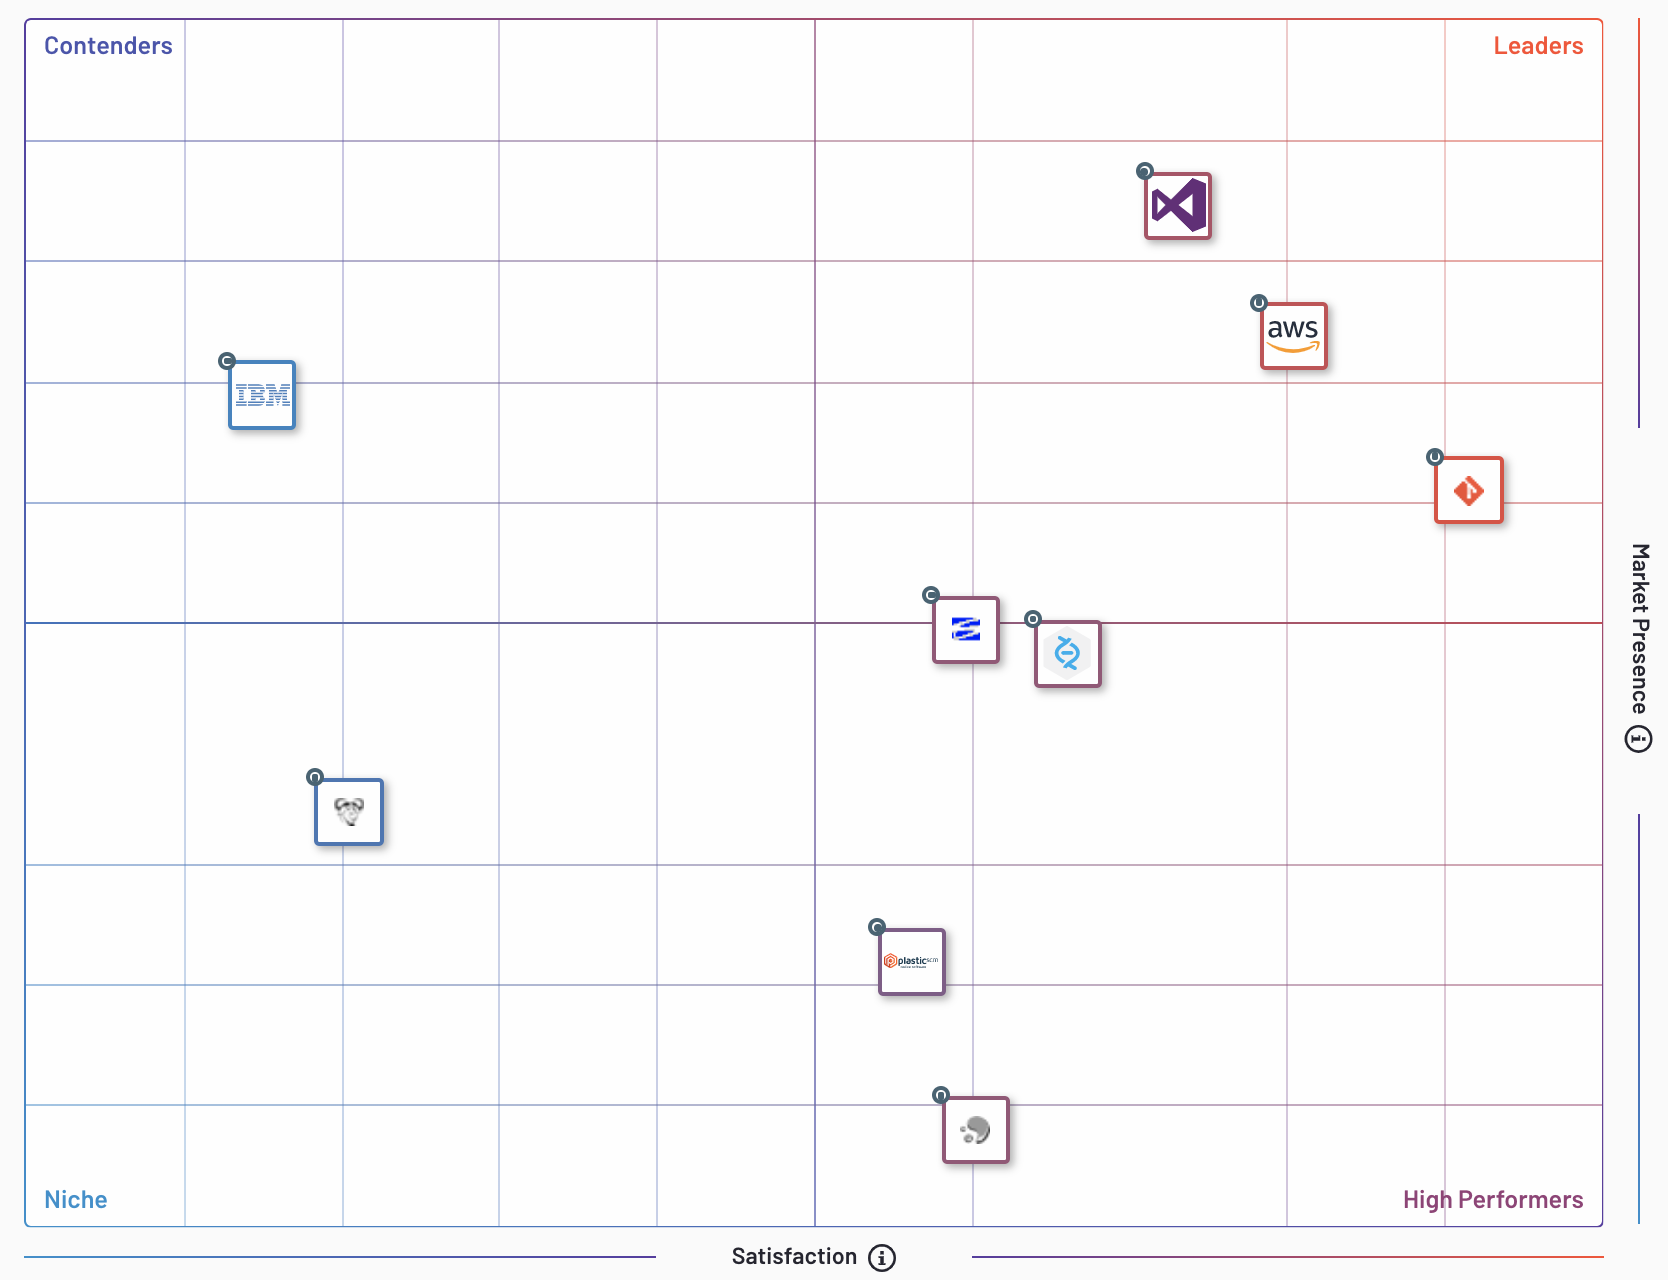
\includegraphics[width=\textwidth]{source-control-high-perf.png}
	\caption{2019 - Best Version Control Systems}
	\label{fig:g2:source-control}
\end{figure}